\documentclass[12pt]{article}
\usepackage[a4paper, margin=1in]{geometry} 
\usepackage{graphicx} 
\usepackage{hyperref}
\usepackage{float}
\usepackage{multicol}
\usepackage{multirow}
\usepackage{amsmath}
\usepackage[ruled]{algorithm2e}
\usepackage{amssymb}
\usepackage[font=small, labelfont=bf]{caption}
\usepackage[table,xcdraw]{xcolor}

\title{Lecture Notes for \\ INF281 Basics of Bioinformatics Sequence Analysis}
\author{Takaya Saito}
\date{}

\begin{document}

\pagenumbering{arabic}
\setcounter{page}{88}

\makeatletter 
\renewcommand{\thefigure}{\arabic{section}.\arabic{figure}}
\renewcommand{\thetable}{\arabic{section}.\arabic{table}}
\makeatother

%
% Sequence profiles
%
\setcounter{section}{11}
\setcounter{figure}{0}
\setcounter{table}{0}
\section{Sequence profiles}
%\documentclass[12pt]{article}
%\usepackage[a4paper, margin=1in]{geometry} 
%\usepackage{graphicx} 
%\usepackage{hyperref}
%\usepackage{float}
%\usepackage{multicol}
%\usepackage{multirow}
%\usepackage{amsmath}
%\usepackage[font=small, labelfont=bf]{caption}
%
%\begin{document}

%
% Sequence profiles and patterns
%
\subsection{Sequence profiles and patterns}

%
% Protein secondary structures
%
\subsubsection*{Protein secondary structures}

\begin{figure}[H]
  \centering
      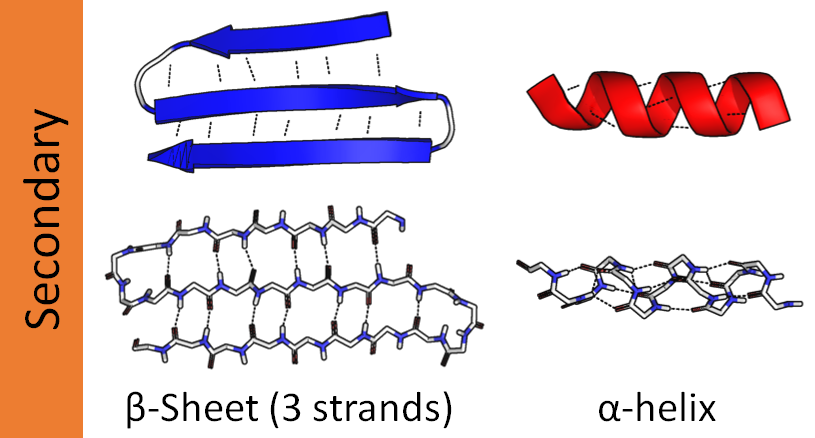
\includegraphics[width=0.5 \textwidth]{fig12/Alpha_beta_structure.png}
  \caption{Protein secondary structures (source: \href{https://commons.wikimedia.org/w/index.php?curid=56202452}{Shafee, Wikimedia Commons})}
\end{figure}

%
% Functional regions found in MSA
%
\subsubsection*{Functional regions found in MSA}

\begin{itemize}
\item \url{http://www.bioinformatics.org/strap/}
\item \url{http://journals.plos.org/plosone/article?id=10.1371/journal.pone.0070843}
\end{itemize}

%
% Applications of MSAs
%
\subsubsection*{Applications of MSAs}
\begin{itemize}
\item Position weight matrix
\item Sequence profile
\item HMM profile
\item Motifs
\end{itemize}

\bigskip 

%\end{document}

%\documentclass[12pt]{article}
%\usepackage[a4paper, margin=1in]{geometry} 
%\usepackage{graphicx} 
%\usepackage{hyperref}
%\usepackage{float}
%\usepackage{multicol}
%\usepackage{multirow}
%\usepackage{amsmath}
%\usepackage[font=small, labelfont=bf]{caption}
%
%\begin{document}

%
% Position weight matrix 
%
\subsection{Position weight matrix }
A position weight matrix (PWM) is a two-dimensional array that contains position-specific scores. PWMs usually contain no gaps.

%
% Creating a position probability matrix (PPM)
%
\subsubsection*{Creating a position probability matrix (PPM)}
It requires an MSA without gaps.

%
% Example of PPM
%
\subsubsection*{Example of PPM}
Make a PPM from the alignment below.

\begin{verbatim}
   Seq1 AGT
   Seq2 CAG
   Seq3 AAT
   Seq4 ATT
\end{verbatim}

\noindent
Position-specific frequencies
\begin{table}[H]
\centering
\begin{tabular}{|l|l|l|l|}
\hline
  & 1 & 2 & 3 \\ \hline
A & 3 & 2 & 0 \\ \hline
G & 0 & 1 & 1 \\ \hline
C & 1 & 0 & 0 \\ \hline
T & 0 & 1 & 3 \\ \hline
\end{tabular}
\end{table}

\noindent
PPM
\begin{table}[H]
\centering
\begin{tabular}{|l|l|l|l|}
\hline
  & 1    & 2    & 3    \\ \hline
A & 0.75 & 0.5  & 0    \\ \hline
G & 0    & 0.25 & 0.25 \\ \hline
C & 0.25 & 0    & 0    \\ \hline
T & 0    & 0.25 & 0.75 \\ \hline
\end{tabular}
\end{table}

%
% From PPM to PWM
%
\subsubsection*{From PPM to PWM}
Similar to pair-wise scores, log-odds scores can be used for profiles. \\ \\

$\begin{aligned}
\mathrm{PWM}_{ar} =& \log \dfrac{\mathrm{PPM}_{ar}}{q_a} \\ \\
q_a :& \text{ Background probability of } a \\
r :& \text{ Position in MSA}  
\end{aligned} $

\bigskip 

%\end{document}

%\documentclass[12pt]{article}
%\usepackage[a4paper, margin=1in]{geometry} 
%\usepackage{graphicx} 
%\usepackage{hyperref}
%\usepackage{float}
%\usepackage{multicol}
%\usepackage{multirow}
%\usepackage{amsmath}
%\usepackage[font=small, labelfont=bf]{caption}
%
%\begin{document}

%
% Sequence profiles 
%
\subsection{Sequence profiles}
A protein sequence profile is a two-dimensional array that contains position-specific scores.

%
% Profile values
%
\subsubsection*{Profile values}
A profile is based on position-specific weights and a score matrix. \\ \\

$\begin{aligned}
\mathrm{Prof}_{ra} :& \text{ Position-specific score of } a \text{ at position } r \\ \\
R_{ab} :& \text{ Pair-wise score of } a \text{ and } b \\
r :& \text{ Position in MSA}  \\
a, b :& \text{ Nucleotide/amino acid element}  \\
M :& \text{ All nucleotides/amino acids}  \\ \\
W_{rb} :& \text{ Weight value of }  b \text{ at position } r 
\end{aligned} $

%
% Profile with linear weights
%
\subsubsection*{Profile with linear weights}

\bigskip 

$\begin{aligned}
\mathrm{Prof}_{ra} =& \dfrac{1}{m_r} \sum_{b \in M}{} R_{ba} F_{rb} \\ \\
W_{rb} =& \dfrac{F_{rb}}{m_{r}} \\
F_{rb} :& \text{ The number of occurrences of } b \text{ at position }  r \\
m_{r} :& \text{ The number of residues without gaps at position } r 
\end{aligned} $

%
% Example of profile with linear weights
%
\subsubsection*{Example of profile with linear weights}

Make a profile with linear weights. \\

\noindent
Alignment
\begin{verbatim}
   Seq1 AGC
   Seq2 -AC
   Seq3 AAT
\end{verbatim}

\medskip 

\noindent
Scoring matrix
\begin{table}[H]
\centering
\small
\begin{tabular}{|c|c|c|c|c|}
\hline
  & A  & G  & C  & T  \\ \hline
A & 2  & 1  & -3 & -2 \\ \hline
G & 1  & 3  & -2 & -1 \\ \hline
C & -3 & -2 & 4  & 1  \\ \hline
T & -2 & -1 & 1  & 2  \\ \hline
\end{tabular}
\end{table}

\noindent
Scores can be calculated as follows. \\

$\begin{aligned}
\mathrm{A1}: & \quad 1/2 \times (2 \times 2 + 1 \times 0 + (-3) \times 0 + (-2) \times 0) = 1/2 \times 4 = 2 \\
\mathrm{G1}: & \quad 1/2 \times (1 \times 2 + 3 \times 0 + (-2) \times 0 + (-1) \times 0) = 1/2 \times 2 = 1 \\
\mathrm{C1}: & \quad 1/2 \times ((-3) \times 2 + (-2) \times 0 + 4 \times 0 + 1 \times 0) = 1/2 \times (-6) = -3 \\
\mathrm{T1}: & \quad 1/2 \times ((-2) \times 2 + (-1) \times 0 + 1 \times 0 + 2 \times 0) = 1/2 \times (-4) = -2 \\ \\
\mathrm{A2}: & \quad 1/3 \times (2 \times 2 + 1 \times 1+(-3) \times 0+(-2) \times 0) = 1/3 \times 5=1.67 \\
\mathrm{G2}: & \quad 1/3 \times (1 \times 2 + 3 \times 1+(-2) \times 0+(-1) \times 0) = 1/3 \times 5=1.67 \\
\mathrm{C2}: & \quad 1/3 \times ((-3) \times 2 + (-2) \times 1+4 \times 0+1 \times 0) = 1/3 \times (-8) = -2.67 \\
\mathrm{T2}: & \quad 1/3 \times ((-2) \times 2 + (-1) \times 1+1 \times 0+2 \times 0) = 1/3 \times (-5) = -1.67 \\ \\
\mathrm{A3}: & \quad 1/3 \times (2 \times 0 + 1 \times 0 + (-3) \times 2 + (-2) \times 1) = 1/3 \times (-8) = -2.67 \\
\mathrm{G3}: & \quad 1/3 \times (1 \times 0 + 3 \times 0 + (-2) \times 2 + (-1) \times 1) = 1/3 \times (-5) = -1.67 \\
\mathrm{C3}: & \quad 1/3 \times ((-3) \times 0 + (-2) \times 0 + 4 \times 2 + 1 \times 1) = 1/3 \times (9) = 3 \\
\mathrm{T3}: & \quad 1/3 \times ((-2) \times 0 + (-1) \times 0 + 1 \times 2 + 2 \times 1) = 1/3 \times (4) = 1.33 \\
\end{aligned} $

\bigskip \bigskip 

\noindent
Calculated profile with linear weights.

\begin{table}[H]
\centering
\begin{tabular}{|c|c|c|c|c|}
\hline
  & A     & G     & C     & T     \\ \hline
1 & 2     & 1     & -3    & -2    \\ \hline
2 & 1.67  & 1.67  & -2.67 & -1.67 \\ \hline
3 & -2.67 & -1.67 & 3     & 1.33  \\ \hline
\end{tabular}
\end{table}

%
% Non-linear weights
%
\subsubsection*{Non-linear weights}
Amino acids/nucleotides occurring many times are ``favored''.

\[
\mathrm{W}_{rb} = \dfrac{ \ln((1-F_b)/(1+m_r)) }{ \ln(1/(1+m_r)) }
\]

\bigskip 

\noindent
Amino acids/nucleotides occurring many times are ``punished''.

\[
\mathrm{W}_{rb} = \dfrac{ 1 + \ln(1-F_b) }{ 1 + \ln m_r }
\]

\bigskip 

\begin{figure}[H]
  \centering
      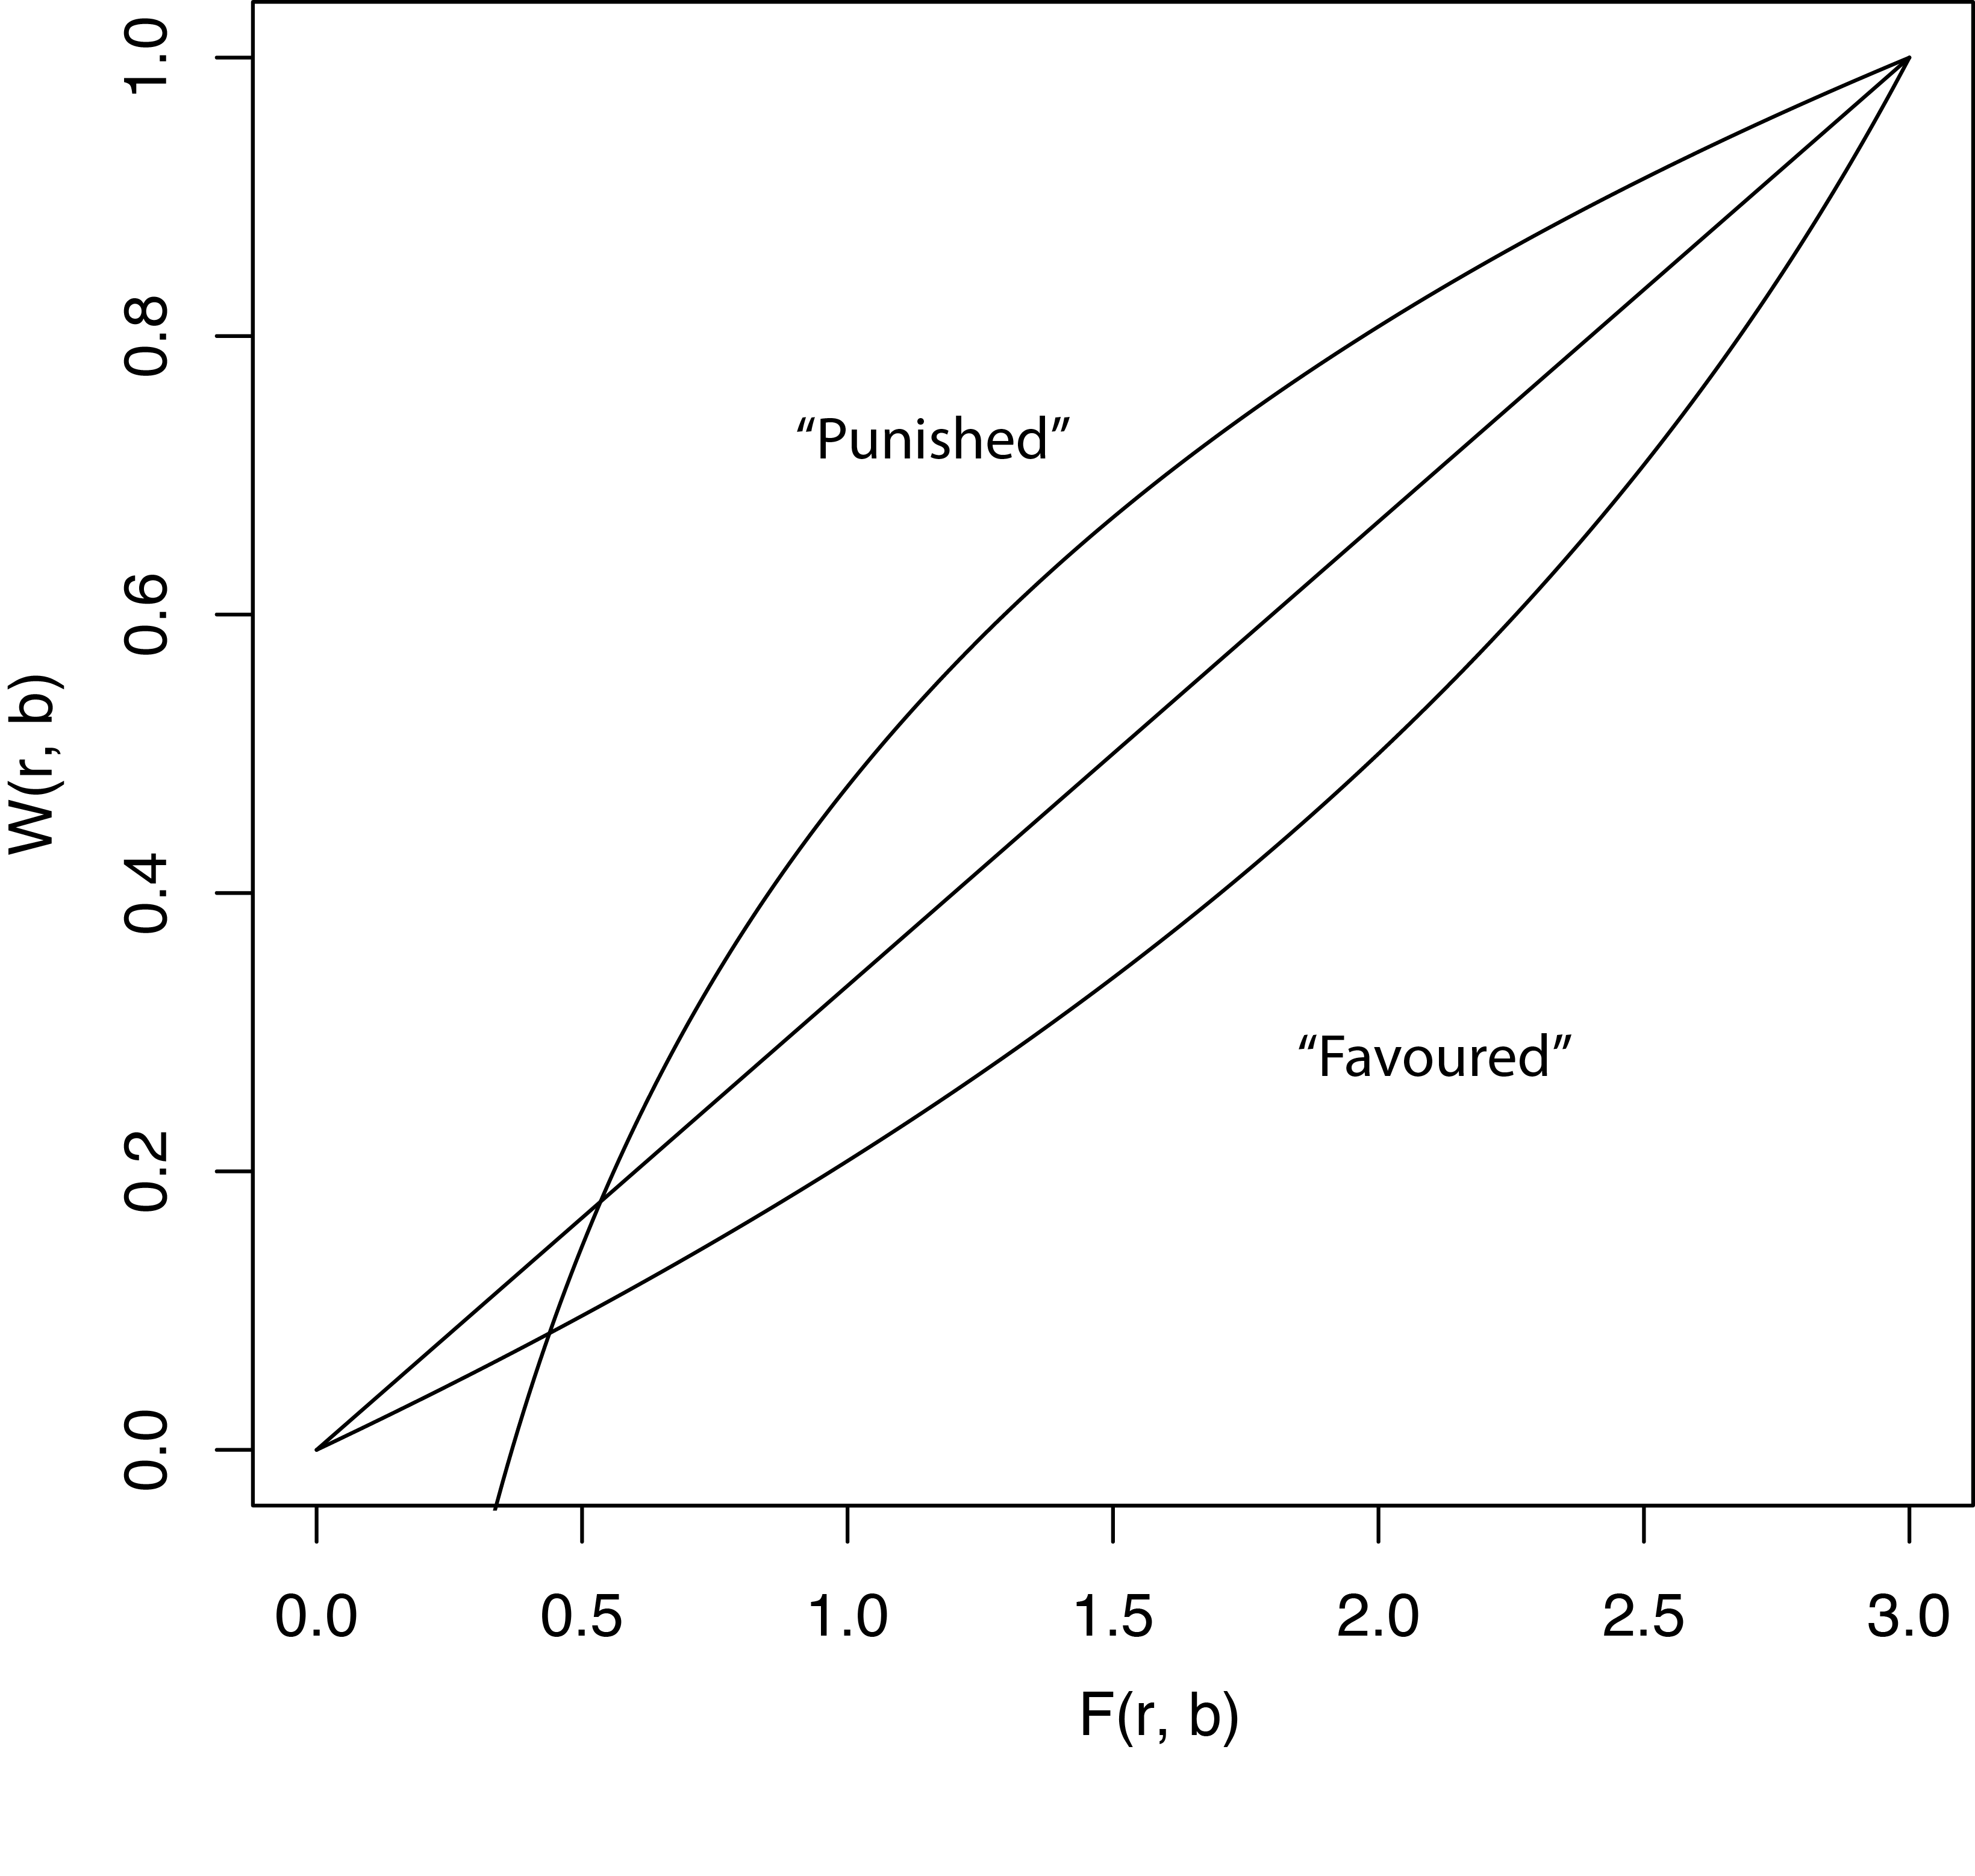
\includegraphics[width=0.3 \textwidth]{fig12/weight_functions.png}
  \caption{Two different weight functions)}
\end{figure}

%
% Treating gaps
%
\subsubsection*{Treating gaps}
Position-specific gap penalties are usually added to profiles.

\bigskip 

%\end{document}

%\documentclass[12pt]{article}
%\usepackage[a4paper, margin=1in]{geometry} 
%\usepackage{graphicx} 
%\usepackage{hyperref}
%\usepackage{float}
%\usepackage{multicol}
%\usepackage{multirow}
%\usepackage{amsmath}
%\usepackage[font=small, labelfont=bf]{caption}
%
%\begin{document}

%
% Profile search
%
\subsection{Profile search}
A constructed profile can be used to find sequence patterns.

%
% Profile score of a query sequence
%
\subsubsection*{Profile score of a query sequence}
The score of a query sequence can be calculated by adding all corresponding position-specific scores.

%
% Example of profile score
%
\subsubsection*{Example of profile score}
Find the best score for q = AGCT. \\

\noindent
Profile:
\begin{table}[H]
\centering
\begin{tabular}{|c|c|c|c|c|c|c|}
\hline
  & A  & G  & C  & T  & Gap & Len \\ \hline
1 & 5  & -5 & -2 & -1 & 10  & 10  \\ \hline
2 & -2 & 3  & 4  & -7 & 10  & 10  \\ \hline
3 & 1  & 2  & 1  & -1 & 5   & 7   \\ \hline
4 & -3 & 3  & -2 & 7  & 10  & 10  \\ \hline
\end{tabular}
\end{table}

\noindent
Score: $5 + 3 + 1 + 7 = 16$

%
% Searching databases with a profile
%
\subsubsection*{Searching databases with a profile}
A dynamic programming method can be used for a profile search. \\

\[
H_{i,j} = \max \left\{0, \mathrm{Prof}_{jd_i} + \max \left\{ \begin{array}{l}
         H_{i-1,j-1} \\
         \max_{2 \ll k \ll j-1} H_{i-1,j-k} - g_k^d  \\
         \max_{2 \ll l \ll i-1} H_{i-l,j-1} - g_l^d  \end{array} \right.  \right. 
\]

\bigskip 

\begin{center}
where $g_k^d$ and $g_l^P$ are database and profile gap penalties.
\end{center}

%
% Example of database search with profile
%
\subsubsection*{Example of database search with profile}
d1 = ACT \\

\noindent
Gap penalty: $5 + 2(l - 1)$ \\

\noindent
Profile:
\begin{table}[H]
\centering
\begin{tabular}{|c|c|c|c|c|c|c|}
\hline
  & A  & G  & C  & T  & Gap & Len \\ \hline
1 & 5  & -5 & -2 & -1 & 10  & 10  \\ \hline
2 & -2 & 3  & 4  & -7 & 10  & 10  \\ \hline
3 & 1  & 2  & 1  & -1 & 5   & 7   \\ \hline
4 & -3 & 3  & -2 & 7  & 10  & 10  \\ \hline
\end{tabular}
\end{table}

\bigskip 

\noindent
DP table:
\begin{table}[H]
\centering
\begin{tabular}{cccccc}
                       &                        & 1                      & 2                      & 3                      & 4                       \\ \cline{2-6} 
\multicolumn{1}{c|}{}  & \multicolumn{1}{c|}{0} & \multicolumn{1}{c|}{0} & \multicolumn{1}{c|}{0} & \multicolumn{1}{c|}{0} & \multicolumn{1}{c|}{0}  \\ \cline{2-6} 
\multicolumn{1}{c|}{A} & \multicolumn{1}{c|}{0} & \multicolumn{1}{c|}{5} & \multicolumn{1}{c|}{0} & \multicolumn{1}{c|}{1} & \multicolumn{1}{c|}{0}  \\ \cline{2-6} 
\multicolumn{1}{c|}{C} & \multicolumn{1}{c|}{0} & \multicolumn{1}{c|}{0} & \multicolumn{1}{c|}{9} & \multicolumn{1}{c|}{5} & \multicolumn{1}{c|}{0}  \\ \cline{2-6} 
\multicolumn{1}{c|}{T} & \multicolumn{1}{c|}{0} & \multicolumn{1}{c|}{0} & \multicolumn{1}{c|}{0} & \multicolumn{1}{c|}{8} & \multicolumn{1}{c|}{12} \\ \cline{2-6} 
\end{tabular}
\end{table}


\begin{table}[H]
\centering
\scriptsize
\begin{tabular}{|l|l|l|l|}
\hline
\multicolumn{1}{|c|}{$\mathrm{H}_{1,1}$: 5} & \multicolumn{1}{c|}{$\mathrm{H}_{1,2}$: 0} & \multicolumn{1}{c|}{$\mathrm{H}_{1,3}$: 1} & \multicolumn{1}{c|}{$\mathrm{H}_{1,4}$: 0}  \\
$\mathrm{Prof_{1A}}$: 5                     & $\mathrm{Prof_{2A}}$: -2                   & $\mathrm{Prof_{3A}}$: 1                    & $\mathrm{Prof_{4A}}$: -3                    \\
\textbf{Diagonal: 5 + 0}               & Diagonal: -2 + 0             & \textbf{Diagonal: 1 + 0}              & Diagonal: -3 + 0              \\
Vertical: 5 + (0 - 10)        & Vertical: -2 + (0 - 10)      & Vertical: 1 + (0 - 10)       & Vertical: -3 + (0 - 10)       \\
Horizontal: 5 + (0 - 5)       & Horizontal: -2 + (5 - 5)     & Horizontal: 1 + (5 - 7)      & Horizontal: -3 + (1 - 5)      \\ \hline
\multicolumn{1}{|c|}{$\mathrm{H}_{2,1}$: 0} & \multicolumn{1}{c|}{$\mathrm{H}_{2,2}$: 9} & \multicolumn{1}{c|}{$\mathrm{H}_{2,3}$: 5} & \multicolumn{1}{c|}{$\mathrm{H}_{2,4}$: 0}  \\
$\mathrm{Prof_{1C}}$: -2                    & $\mathrm{Prof_{2C}}$: 4                    & $\mathrm{Prof_{3C}}$: 1                    & $\mathrm{Prof_{4C}}$: -2                    \\
Diagonal: -2 + 0              & \textbf{Diagonal: 4 + 5}              & Diagonal: 1 + 0              & Diagonal: -2 + 1              \\
Vertical: -2 + (5 - 10)       & Vertical: 4 + (0 - 10)       & Vertical: 1 + (1 - 10)       & Vertical: -2 + (0 - 10)       \\
Horizontal: -2 + (0 - 5)      & Horizontal: 4 + (0 - 5)      & \textbf{Horizontal: 1 + (9 - 5)}      & Horizontal: -2 + (9 - 7)      \\ \hline
\multicolumn{1}{|c|}{$\mathrm{H}_{3,3}$: 0} & \multicolumn{1}{c|}{$\mathrm{H}_{3,2}$: 0} & \multicolumn{1}{c|}{$\mathrm{H}_{3,3}$: 8} & \multicolumn{1}{c|}{$\mathrm{H}_{3,4}$: 12} \\
$\mathrm{Prof_{1T}}$: -1                    & $\mathrm{Prof_{2T}}$: -7                   & $\mathrm{Prof_{3T}}$: -1                   & $\mathrm{Prof_{4T}}$: 7                     \\
Diagonal: -1 + 0              & Diagonal: -7 + 0             & \textbf{Diagonal: -1 + 9}             & \textbf{Diagonal: 7 + 5}               \\
Vertical: -1 + (0 - 10)       & Vertical: -7 + (9 - 10)      & Vertical: -1 + (5 - 10)      & Vertical: 7 + (0 - 10)        \\
Horizontal: -1 + (0 - 5)      & Horizontal: -7 + (0 - 5)     & Horizontal: -1 + (0 - 5)     & Horizontal: 7 + (8 - 5)       \\ \hline
\end{tabular}
\end{table}

\noindent
Alignment:
\begin{verbatim}
   profile: 1234
        d1: AC-T
\end{verbatim}

\bigskip 

%\end{document}

%\documentclass[12pt]{article}
%\usepackage[a4paper, margin=1in]{geometry} 
%\usepackage{graphicx} 
%\usepackage{hyperref}
%\usepackage{float}
%\usepackage{multicol}
%\usepackage{multirow}
%\usepackage{amsmath}
%\usepackage[ruled]{algorithm2e}
%\usepackage[font=small, labelfont=bf]{caption}
%
%\begin{document}

%
% PSI-BLAST
%
\subsection{PSI-BLAST}
Position-specific iterated BLAST  (PSI-BLAST) is an extension of BLAST. It is much more sensitive than BLAST. It can be used to find distantly related proteins.

var
q: query sequence
t: threshold for significance

%
% Simplified procedure of PSI-BLAST
%
\subsubsection*{Pseudo-code of linear progressive alignment (general progressive alignment)}

\begin{algorithm}[H]
  \SetKwInOut{Q}{$\mathrm{q}$}
  \SetKwInOut{T}{$\mathrm{t}$}
  \SetKwRepeat{Do}{do}{while}
  
  \BlankLine
    
  \Q{query sequence}
  \T{threshold for significance}
  
  \BlankLine \BlankLine
  
   Q = BLAST(q, t);

  \BlankLine \BlankLine

  \Do{\textsf{\upshape convergence(Reduce(Q) = Q1) or maximum number of cycles}}{
     Q1 = Reduce(Q);               \tcp*{Remove identical segments}
     M  = MultipleAlignment(Q1); \\
     P  = Profile(M); \\
     Q  = ProfileSearch(P);
  }

  \BlankLine   \BlankLine
  
  \SetAlgoRefName{\thesection.1}
  \caption{Simplified procedure of PSI-BLAST}

\end{algorithm}

\bigskip 

%\end{document}


\end{document}
